
%%%%%%%%%%%%%%%%%%%%%% Title %%%%%%%%%%%%%%%%%%%%%%%%%%

%\documentclass[twocolumn]{article}
\documentclass[a4paper,11pt]{article}
\newcommand{\horrule}[1]{\rule{\linewidth}{#1}} % Create horizontal rule command with 1 argument of height

%\setlength{\topmargin}{20in}
%\titlespacing{\section}{0pt}{0pt}{0pt}

\title{
\normalfont \normalsize
\textsc{Imperial College London\\
MRes in Medical Robotics and Image Guided Intervention} \\ [1pt] % Your university, school and/or department name(s) 
\horrule{0.5pt} \\[0.4cm] % Thin top horizontal rule
\huge Individual Research Project \\
Platform for Microrobot Navigation \\ % The assignment title
\horrule{2pt} \\[0.1cm] % Thick bottom horizontal rule
}
\author{
        Nafiseh Vahabi\\
	Supervisors: Prof Guang-Zhong Yang, Dr Henry lp and Dr Vincenzo Curto
}

%\date{\today}

%%%%%%%%%%%%%%%%%%%%%%%%%%%%%%%%%%%%%%%%%%%%%%%%%%
\usepackage[a4paper]{geometry}
\usepackage[round]{natbib}
\usepackage[pdftex]{graphicx}
\usepackage{amsmath}
\usepackage{multirow} 
\usepackage {fullpage}
\usepackage[inference,shorthand]{semantic}
\usepackage{fancyvrb}
\usepackage{listings}
\usepackage{comment} 
\usepackage{fancyhdr}
\usepackage{url}
\usepackage{subfigure}
\usepackage[english]{babel}
\usepackage{balance}
\usepackage[compact]{titlesec}
\usepackage{sidecap}
\usepackage{wrapfig}


%\renewcommand{\textfraction}{0.1}
%\renewcommand{\floatpagefraction}{0.9}


%%%%%%%%%%%%%%%%%  Hyphenate  %%%%%%%%%%%%%%%%%%

\hyphenpenalty=2500

%%%%%%%%%%%%%%%%%%%%%% Page layout %%%%%%%%%%%%%%%%%%%%%%

%\fancyhead{}
%\fancyhead[LO,RE]{\slshape \leftmark}
\fancyfoot[C]{\thepage}
\fancyhead{} % clear all header fields
\renewcommand{\headrulewidth}{0.4pt}
\renewcommand{\footrulewidth}{0.4pt}
%\pagestyle{fancy}
\rhead{ Platform for Microrobot Navigation}

%\fancyhead[CO,CE]{---Draft---}
%\fancyfoot[C]{Confidential}
%%%%%%%%%%%%%%%%%%%%%%%%%%%%%%%%%%%%%%%%%%%%%%%%%%%%

\begin{document}
%\newgeometry{top= 1.5 cm}
%\newgeometry{bottom= 1.5 cm}


%\addtolength{\oddsidemargin}{-.875in}
%	\addtolength{\evensidemargin}{-.875in}
%	\addtolength{\textwidth}{1.75in}
%\addtolength{\topmargin}{-.875in}
%	\addtolength{\textheight}{1.75in}

\begin{sloppypar}


\maketitle
\thispagestyle{plain}

%\begin{abstract}
%This is abstract
%\end{abstract}

%%%%%%%%%%%%%%%%%%%%%%%%%%  INTRODUCTION  %%%%%%%%%%%%%%%%%%%%%%%%%%
\section{Introduction}

In the recent years, researchers were interested in magnetically actuated helical micromechanisms for use
 in a variety of biomedical applications such as cell characterisation, targeted drag delivery and vivo 
diagnosis ~\citep{peyer2013magnetic}. However, the extremely small size of the microrobots and the biofluid environment make the design 
very challenging. The two main difficulties are the power supply and finding suitable locomotion methods, as
 there are many cells, proteins and fibres in biofluids that prevent the motion of the microrobots. 
The common method of using an external magnetic field produced the most succesful result ~\citep{peyer2013bio}. 
\paragraph{}


%\restoregeometry. 

%%%%%%%%%%%%%%%%%%%%%%%%%  Literature review  %%%%%%%%%%%%%%%%%%%%%%%%%%%
\section{Literature Review}

The design of microrobots depends on their application and the desired task. Therefore the number of microbots
were designed can be categorised into following groups. 

\paragraph{}
\subsection{Microscrew Like Structure and Actuation Principle}
\paragraph{}
\subsubsection{Helical Shape}

 There is three common shapes of microrobots 
based on the rotary action; a helix, a screw and a twisted ribbon shape around its axis(Figure~\ref{HelixShapes}). 


For the purpose of drilling into solid matter the screw and helix design would be more appropriate.
 However for the helical shape there is one pitch per rotation. There is also the consideration of penetrating
 a solid material from a fluidic environment. In the solid material, the rear part of the helical device will shift 
into the same location as the front part. In the fluidic regime this is not the case because of the low
 Reynolds number~\citep{peyer2013magnetic}. The Reynolds number describes the ratio of the inertial forces versus viscous 
forces according the following formula;

\begin{equation}
  Re = \cfrac{UL\rho}{\mu}
\label{eq:4}
\end{equation}
 
Where $ U$ is velocity, $L$ is characteristic length, $\rho$ is the density and $\mu$ is viscosity of the fluid.
The very small length $(L)$ and velocity $(U)$ of the microrobots results in the very small Re $(Re\ll1)$. 
The motion in the environment with such a low Re can be described as being similar to a human
 trying to swim and move in honey. In the case of the helical microdevice, the helical rotation will not move 
forward in the same way as in solid matter because whilst the device is rotating in a fluid environment, 
it only moves by a small percentage of its pitch length per rotation ~\citep{peyer2013magnetic}. 

%\begin{figure}
%\begin{SCfigure}
  %\centering
\begin{wrapfigure}{r}{0.5\textwidth}
  \begin{center}
    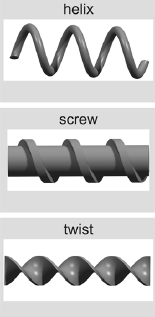
\includegraphics[width=0.4\textwidth]{HelixShapes}
  \caption{Three design of helical microswimmers.~\citep{peyer2013magnetic}.}
  \label{HelixShapes}
  \end{center}
\end{wrapfigure}
%\end{SCfigure}
%\end{figure}

\paragraph{}
 For the purposes of drug delivery the tabular and helical lipid microstructure was successful
 and had good loading capacity and propulsion efficiency. The rotational motion of helical micro
 swimmers is one of the most effective propulsion methods in the low Reynolds number scenarios 
because it leads to translational motion. Microrobots with the microspheres structure perform similarly 
to the helical swimmers and are capable of swimming in the flowing liquid in microfluidic channel ~\citep{kim2013fabrication}. 
More recently, a three-dimensional porous micro-niches designed for cell transportation purposes used
 photocurable polymer for its fabrication method. To improve biocompatibility for in-vivo application, the 
microrobot can be covered with a thin layer of titanium. In addition, the structures were layered with 
nickel for the purpose of magnetic actuation. A magnetic manipulator rotates and translates the 
microrobot wirelessly. Most in-vivo environments are three-dimensional, hence the 3D navigation will be 
required for the successful microrobot ~\citep{kim2013fabrication}.
One of the porous 3D structures used for cell adhesion and organ regeneration is called scaffold. 
Porous structures with the controllable porosity demonstrate improved characteristic such as high cell 
compactness and uniform cell distribution in comparison with the scaffold structure. Three-dimensional 
laser lithography is a state of the art technique to fabricate bio-scaffold structures (Figure~\ref{ref4}). In this method a building unit is a 
single ellipsoidal spot, which form as a result of concentration of two laser beams. A pre-programmed path 
is followed by controlling the movement of a piezoelectric stage precisely to partly expose the photoresist.
 After removing the unexposed photoresist a complete three-dimensional structure of the microrobot can 
be formed.   

%\begin{figure}
%\begin{SCfigure}
\begin{wrapfigure}{r}{0.5\textwidth}
  \begin{center}
  \centering
    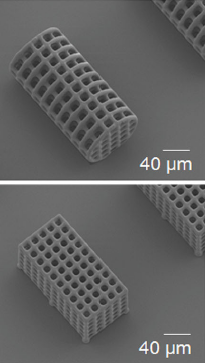
\includegraphics[width=0.4\textwidth]{4}
  \caption{The image of two designs of fabricated microrobot under scan electron microscopy, cylindrical-shaped (first)
and hexahedral-shaped (second) ~\citep{kim2013fabrication}.}
  \label{ref4}
\end{center}
\end{wrapfigure}
%\end{SCfigure}
%\end{figure}

There are two main factors that affect the movements of the microrobot in the external magnetic
 field; low coercivity and high saturation magnetization. Also, the motion of the microrobot is related to 
its size given the same magnetic field and as such, by increasing the size of the microrobot with the inflexible magnetic material
 volume, the velocity will decrease ~\citep{kim2013fabrication}. 
The surface friction and the drag forces are two resistive forces that impede the microrobot 
motion. Hence, the input magnetic force must be sufficient to overcome these forces for microrobot 
manipulation. Furthermore, the weight of the microrobot required compensating in the z-direction by 
the magnetic field. The mathematic model below describes the microrobot translational movement;

\begin{equation}
  \overrightarrow{F_m }+ \overrightarrow{F_r} - \overrightarrow{F_g} = m(\overrightarrow{dv}/dt)
\label{eq:4}
\end{equation}

Where $F_m$, $F_r$ and $F_g$ are a magnetic force, overall resistive force and gravitational force respectively. 
$M$ is a mass and $v$ is a translational velocity of the microrobot~\citep{kim2013fabrication}.  

Hexahedral microrobot and cylindrical microrobot can be developed using a similar method (Figure~\ref{ref4}).
 However, because nickel is deposited uniformly on the surface of these microrobots, the 
Hexahedral structure has a greater amount of nickel deposited on its surface. Consequently, the 
magnetic force required for the hexahedral microrobot is greater than the cylindrical one while its 
translational velocity is lower than the cylindrical microrobots. Hence, the cylindrical structure is preferable
 for the purpose of minimising the resistive force against manipulation ~\citep{kim2013fabrication}. 

A magnetic field can be used for controlling teams of microrobots as well as a single 
one. \citeauthor{kim2013fabrication} proposed a method that used a combination of two magnetic materials to 
attain on/off magnetization of each microrobot. The overall control of the group of microrobots 
was achieved by managing the state of each agent. In addition, a second technique has been 
developed for three-dimensional motion of the team of microrobots in a fluidic environment. In
 the latter method, each microrobot is designed in such a way that it uniquely responds to the 
same input magnetic filed. Therefore, several microrobots can provide feedback position control in 
3D system~\citep{kim2013fabrication}.
An untethered spherical magnetic micromanipulator creates a locally induced rotational fluid flow field. 
The created rotational flow propels micro-objects in the flow area. The ream of microrobot could perform
 a complex task in micro-transport and micro-assembly~\citep{kim2013fabrication}.

\paragraph{}
In another study ~\citep{tottori2012magnetic}, a helical microrobot designed to swim in a low Reynolds number fluid, a 3D 
direct laser writing method was applied as the preferable technique for fabrication. This fabrication 
method allows flexible design of microrobot in which two designs are selected to run the experiment 
and demonstrate the result. The first structure is a bare helical structure and the second one is the
 helical shape with the microholder attached at the end. Both designs will generate the corkscrew
 motion in a fluid environment when there is sufficient magnetic filed. The second 
design (device with the microholder) is capable of transporting a microobject accurately to the 
target ~\citep{tottori2012magnetic}.
The fabrication process consists of the three stages that are fairly similar to the work
 performed by ~\citeauthor{kim2013fabrication}. In the first step, direct laser writing in negative tone photoresist 
wrote the helical device. The developer then removed the unpolymerized photoresist. Finally, the 
developed helical swimmers were left for drying out and then coated in a thin layer of titanium and 
nickel for biocompatibility and magnetic actuation ~\citep{tottori2012magnetic}.

In ~\citeauthor{tottori2012magnetic} experiment eight different designs of microrobots were proposed and tested. 
The uniform static magnetic field was used to explore the magnetic shape anisotropy and the 
magnetic actuation was monitored in the rotating magnetic field. In the static magnetic field the 
set of microrobots with the helical angles ranging from ${45^{\circ}}$ to ${70^{\circ}}$ were suspended in the deionised water. 

%\begin{figure}
  %\centering
\begin{wrapfigure}{r}{0.5\textwidth}
  \begin{center}
    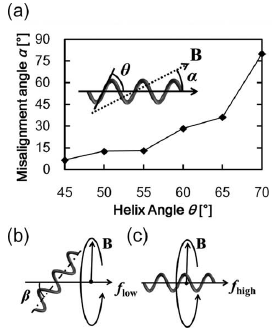
\includegraphics[width=0.5\textwidth]{7}
  \caption{(a) The misalignment of helical angle$\alpha$ with differnt helix angle (b) the oscillation behaviour
of the microswimmer with the high and low frequencies ~\citep{tottori2012magnetic}.}
  \label{ref7}
\end{center}
\end{wrapfigure}
%\end{figure}

This showed (Figure~\ref{ref7}) that a smaller helix angle $\theta$ results in a less misalignment 
angle $\alpha$ because microrobots longest axes will be aligned to the direction of the external magnetic field. 
However in helical microrobot with the larger helix angles the magnetization direction would change to 
the radial axes of the helix  ~\citep{tottori2012magnetic}.
In the rotating magnetic field, the micro helical swimmer exhibits different behaviours depending on 
the strength of the applied frequency in the fixed magnetic field. At low frequencies the micro helix wobbled 
around the helical axes, however by increasing the frequency the oscillating behaviour changed to the 
corkscrew motion. This is similar to characteristics observed on the microrobots with the incorporated
 microholder  ~\citep{tottori2012magnetic}. 

The velocity of helical micro swimmers depends on their size and shape. The linear relation was 
observed between the input frequencies and swimming velocity of the micro swimmers. The outcome of 
the comparison between three microhelixs with the same helix angles showed that the microhelix with the
 greatest diameter has the highest speed, in accordance with the following formula;

\begin{equation}
  U = {\cfrac{(C_n - C_1) \sin \theta \cos \theta}{2(C_n \sin^2 \theta + C_1 \cos^2 \theta)}} \big( d \varpi \big)
\end{equation} 

Where $C_n$ is a drag coefficient perpendicular to the filament and $C_1$ is a drag coefficient
 parallel to the filament. $ \varpi$ is the rotational frequency and $d$ is the rotational diameter of 
the helix ~\citep{tottori2012magnetic}.  



\paragraph{}
The important role of helix angle in the magnetization structure of helical micro swimmers 
was confirmed by \citeauthor{peyer2013bacteria}, who again used direct laser writing as a fabrication method but 
applied that on the magnetic polymer composite (MPC). The MPC are non-cytotoxic and showed 
super paramagnetic characteristic because magnetic material was already included in the polymer. 

The relationship between the torque $T_d$, the drag force $F_d$, the object\rq{}s velocity $U$ and rotational 
speed $\omega$ is linear and modelled by $6\times6$ resistant matrix as below;



\[
\begin{bmatrix} F_d \\ 
T_d \end{bmatrix}  =- \begin{bmatrix} A & B \\ 
B^T & C \end{bmatrix}  \begin{bmatrix} U
 \\ \Omega
\end{bmatrix}
\]




Where $A$, $B$ and $C$ are matrices 3x3 and only depends on the object\rq{}s geometry and fluid velocity. 
There are few methods in use to model the resistance matrices and low Reynolds flow such as the 
method of regularized stokeslets, the boundary element method and the method of fundamental solution
. In designing a microrobot the main parameters required to concentrate on are the helicity angle $\psi$, 
the helix radius $R$, the pitch $p$ and the filament radius $r$ as can shown in Figure~\ref{ref8} part (c). 

\begin{figure}
  \centering
    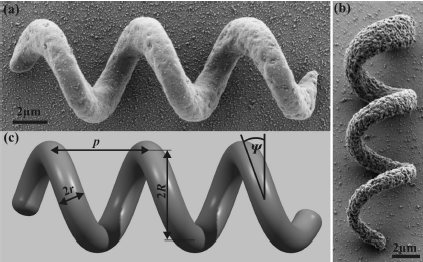
\includegraphics[width=0.7\textwidth]{8}
  \caption{ The prototype of microhelical device. (a) Scanning electron microscopic image of the micro polymer composit
with the 2 vol.\% nanoparticle fill factor and (b) 4 vol.\% of nanoparticle fill factor. (c) The CAD model
shows all the parameters required for the microhelical design ~\citep{peyer2013bacteria}.}
  \label{ref8}
\end{figure}


The micro robot using torque-driven method is more favourable than the force-driven method 
because their rotation is based on applying torque rather than a force to pull the device ~\citep{peyer2013bacteria}. 

\paragraph{}
One of the problems with a man-made nature inspired micro device is that they are 
usually heavier than their natural counter part. In the case of microrobots, the navigation methodology should compensate for gravity to avoid sinking and enable velocity to be 
controlled wirelessly. \citeauthor{mahoney2011velocity} described an algorithm for helical microswimmers velocity 
control plus gravity compensation. In the proposed model the correct pitch angel and 
rotation speed is calculated to achieve the commanded velocity~\citep{mahoney2011velocity}.

\begin{figure}
  \centering
    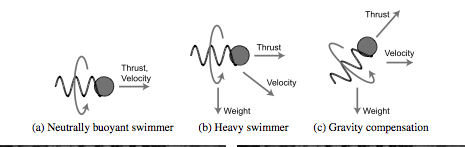
\includegraphics[width=0.9\textwidth]{11}
  \caption{The effect of the gravity on the microrobot motion direction and gravity compensation .~\citep{mahoney2011velocity}.}
  \label{11}
\end{figure}



\paragraph{}
\subsubsection{Tube Shape}

%\begin{figure}
%  \centering
\begin{wrapfigure}{r}{0.5\textwidth}
  \begin{center}
    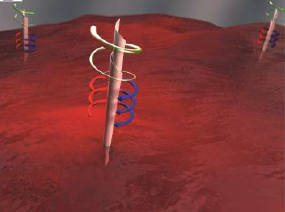
\includegraphics[width=0.5\textwidth]{nanoJet3}
  \caption{Magnetic microtube. Demostrating the drilling motion of the nanotubes under rotating
 magnetic field~\citep{C2NR32798H}.}
  \label{nanotube}
\end{center}
\end{wrapfigure}
%\end{figure}

Another approach for powering a micro robot is using the catalytic conversion of chemical energy
 into mechanical energy (Figure~\ref{nanotube}). In this method, the catalyst accelerates the disintegration of hydrogen peroxide
 and helps the self-propulsion of micro robot to pump the fluid to transport cells and colloidal 
particles ~\citep{C2NR32798H}.
The catalytic tube (nanotube) is fabricated with a sub micrometer diameter.
 This technique is not applicable for the minimally invasive surgery (MIS) yet because the catalytic
 material used in the fabrication process of nanotubes is toxic and sustain viable mammalian cellular 
functions. Hence, biocompatible fuel is required to be developed in order to apply this technique in the 
live cell ~\citep{C2NR32798H}.
Alternatively, the micro driller can be powered and controlled by using an external magnetic field 
such that changes in the frequency of the rotating magnetic field switch the rotational orientation of the 
micro tool from the horizontal position to the vertical one. The vertical orientation of the rolled up microtube 
and its sharp helical design makes the device suitable for drilling into biological tissue. In addition, the micro 
driller can be used for targeted drug delivery in MIS ~\citep{C2NR32798H}. 




\subsection{Bioinspired Flagella (tail) Propulsion Microbots}

One of the most challenging aspects of designing a robot on a very small scale such 
as a nanorobot is simplicity. The reason is, integration will become unfeasible on that
 scale if the design is complex, hence the development of the nanorobot or even microrobot
 should be based on the essential functionality, avoiding any unnecessary components. Helical 
flagella and cilia are two well-known microswimers in nature that their functionality employed for motion 
generation in artificial microrobots  (Figure~\ref{cilia}). Their motion generation mechanism relies on
 the drag imbalance of a cylindrical element and non-reciprocal motion ~\citep{gao2013bioinspired}. 



\begin{figure}
  \centering
    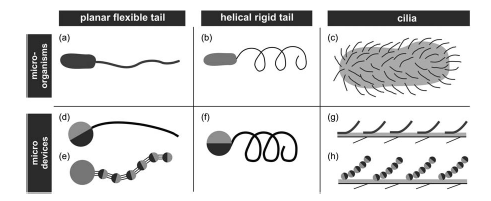
\includegraphics[width=0.9\textwidth]{cilia}
  \caption{The illustration of both flagellum and cilia shapes and microdevices mimicked the flagellum and cilia 
structures.~\citep{peyer2013bio}.}
  \label{cilia}
\end{figure}

In 2007, Bell ~\citep{gao2013bioinspired}presented the first artificial bacteria flagellum microrobots and then
 Zhang characterised them in 2009 ~\citep{gao2013bioinspired}. This artificial microrobot was formed of two 
components; a rigid helical tail and a soft magnetic metal head. The head diameter 
was $2.8 \mu  m$ and its length was $30-100 \mu m$. The size of the head is $200 nm$ thicknesses and its 
length varied from $2.5 to 4.5 \mu m$. Since then, other scientists proposed a slightly different design 
structure, that all have the rigid helical tail structure. However, in some cases the magnetic
 materials is used in the device tail rather than the head ~\citep{gao2013bioinspired}. 
However, the fabrication of the microrobot was the main problem that recent fabrication methods 
offer a feasible solution for ~\citep{gao2013bioinspired}. 

There are a number of helical micro propellers that used external magnetic fields successfully and their
 method has been published but they usually require a complex setup ~\citep{qiunanohelices}. 
By learning from nature and mimicking the structure of live organisms, we can create successful  
scientific applications. 
The helical rotation of flagella and the travelling wave beat of cilia are two non-reciprocal propulsion
 mechanisms in microorganisms. Mimicking a rotating flagellum at low Reynolds number to generate an 
adequate torque to overpower the high viscous drag requires two main elements; a rotary motor and a
 power source ~\citep{qiunanohelices}. 
An electromagnetic rotary motor can be used in designing the helical flagella style microrobot that 
required a considerable current. However piezoelectric rotary motors are an alternative option 
that fit for miniaturisation but necessitate high input voltage.  Hence, designing a microrobot with a 
combination of onboard powering source and motor is a challenging task ~\citep{qiunanohelices}.

\paragraph{}
Another design of microswimmers was inspired by the function of magtigonemes in nature ~\citep{tottori2013artificial}.
 A smooth flagellum moves against the direction of the propagation of the flagellar wave. However, 
the flagellum covered by magtigoneme propels in the same direction as the flagellum wave (Figure~\ref{10}). Mimicking 
the structure of flagellum and using 3D lithography and electron beam evaporation formed the fabrication 
method in this microswimmers.

The anisotropic viscous drag on flagella is an important fact for locomotion in low Reynolds number fluid. 
Flagella movement in the opposite direction of the flagella wave can be explained by this factor so as the 
viscous drag coefficient perpendicular to the flagella is greater than the viscous drag coefficient parallel to 
the flagella ~\citep{tottori2013artificial}. 
The fabrication process consists of two stages. Initially the core structure of the artificial helical 
microswimmer is printed using 3D lithography and then electron beam evaporation is used for 
ferromagnetic thin film coating ~\citep{tottori2013artificial}.  

%\begin{figure}
%  \centering
\begin{wrapfigure}{r}{0.5\textwidth}
  \begin{center}
    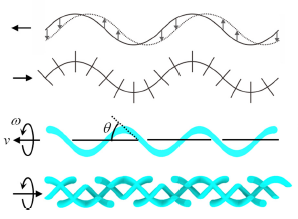
\includegraphics[width=0.5\textwidth]{10}
  \caption{ The structure of the smooth flagellum and a mastigonemes flagellum.~\citep{gao2013bioinspired}.}
  \label{10}
\end{center}
\end{wrapfigure}
%\end{figure}


Performance of each microswimmers (with different design) can be scanned by the scanning electron
 microscope (SEM). After the fabrication process is completed, the next step is releasing the structure in 
the deionised water using the tungsten probe. The tank with deionised water is installed in the middle of the 
three-axis Helmholtz setup.  The rotating field, i.e. rotational frequency, field strength and angles that 
defined the rotational axis can control by the current in the coil. The helical microrobots rotate 
synchronously with the rotation of the magnetic field and move forward and backward accordingly ~\citep{tottori2013artificial}. 


The displacement of the microswimmer along the rotational axis can be measured and the result 
used to calculate the average velocity of the swimmers. There is a linear relationship between an input 
field frequency and swimming speed. According to their result ~\citep{tottori2013artificial}, a propulsive force generated by 
the mastigoneme is in opposite direction of the force generated by the main helical filament. 


The swimming velocity of a mastigoneme helical swimmer is illustrated in  (Figure~\ref{10}) and can be estimated by the following
 symmetric propulsion matrix;


\[
\begin{bmatrix} F\\ 
T \end{bmatrix}  =\begin{bmatrix} A & B \\ 
B & C \end{bmatrix}  \begin{bmatrix} \nu
 \\ \varpi
\end{bmatrix}
\]

Which angular velocity is $\varpi$, valocity $\nu$, external torque $T$ and external force $F$.
The propulsion matrix has two main components; one is for the main flagellum and the second is for the mastigonemes. 
After solving both part of the propulsion matrix,
 the velocity of the microswimmers is given by the equation below;


\begin{equation}
  \nu = {\cfrac{(B_1 + B_2)}{A_1+A_2}} \big( \omega)
\end{equation} 

Where

\begin{equation}
\begin{split}
  A = A_1+A_2 \\
 B= B_1+B_2
\end{split}
\end{equation} 

However, this velocity is only valid if the external force is zero. The proposed 
design ~\citep{tottori2013artificial} is rigid and an external stimulus may be used to regulate the swimming
 speed and direction if the swimmer can fold and unfold their structure. 


\subsection{Scaffold Microbots}


\subsection{Plant-based Microbots}

The helical microstructures are not limited to having flagellum-like structures and microbots with
general cilia-like feature have been designed. \citeauthor{gao2013bioinspired}
 observed the helical microstructures that imitates spiral water-conducting vessels of different plants. 

\begin{figure}
  \centering
    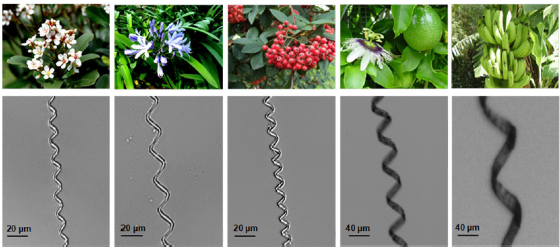
\includegraphics[width=0.9\textwidth]{plants}
  \caption{The shape of the Xylem in differnt plants .~\citep{mahoney2011velocity}.}
  \label{plants}
\end{figure}



The fabrication process involves coating isolated spiral xylem vessel plant fibres within a (Figure~\ref{ref8})
thin magnetic layer. Xylem tissue transports the plant\rq{}s required food such as water and other 
nutrition from the root to the leaves all through capillary action ~\citep{mahoney2011velocity}.
Use of plant material in this method result in simple three-dimensional microswimmers fabrication 
and biocompatibility. In addition, the magnetic cover helps to ensure accurate directional control and 
high-speed propulsion. Therefore the fabrication processes were extremely simplified as the main 
component of the helical microswimmers is from nature and more than a million individual micro helical 
can be made from a very small section of the plant stalk ~\citep{mahoney2011velocity}. 


%\begin{figure}
%  \centering
\begin{wrapfigure}{r}{0.5\textwidth}
  \begin{center}
    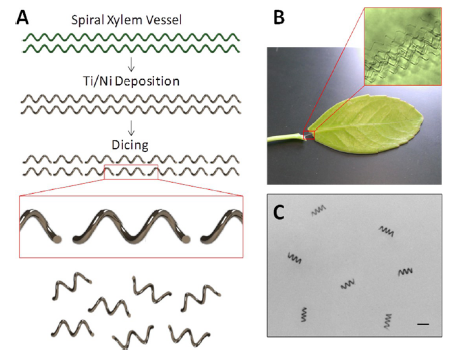
\includegraphics[width=0.5\textwidth]{plants2}
  \caption{The shape of the Xylem in differnt plants ~\citep{gao2013bioinspired}.}
  \label{plants2}
\end{center}
\end{wrapfigure}
%\end{figure}


Using mechanical stretching can control geometric variables of the helical vessels such as the pitch and
 helix angle and hence plentiful helical microswimmers can be reproduced. The final shape of the 
helical microswimmer is determined mainly by the initial diameter of the unstretched spiral vessel. The
 process of stretching helical plant structure was performed via plastic deformation so that the number 
of helical turns are constant and tensile stretching of the plant fibre stretching is negligible~\citep{mahoney2011velocity}. 

The method used for precise propulsion control and characterising the locomotion behaviour of the 
plant-based microswimmers is similar to the method applied in \citeauthor{gao2013bioinspired} study.

According to \citeauthor{gao2013bioinspired} experiment, the plant-based 
microswimmers exhibited high speed movement in raw biological medium such as 
pure human serum under the rotating magnetic field. Moreover, the increased velocity of the 
biological fluid has a minor effect on the plant-driven microswimmers, whichis an important 
advantage of this microdevice over the common microrobots.



\subsection{Bioinspired Jellyfish}
Jellyfish-like swimming robot is another robot design that scientists were interested 
in because of its unique swimming style. Different type of actuators are used to model
 jellyfish-like swimming robot such as shape memory alloy, ionic polymer metal 
composite. However, these jellyfish-like robots were unable to swim freely in 
three-dimensional space due to small propulsion force and were restricted from
 the power supply wire. Therefore an external magnetic field was applied to compensate 
for this power wire issue ~\citep{ko2012jellyfish}.

\begin{figure}
  \centering
    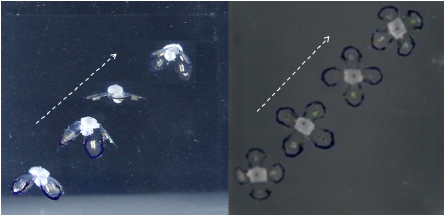
\includegraphics[width=0.9\textwidth]{jellyfish}
  \caption{ The illustration of microrobot\rq{}s locomotion from top and side view ~\citep{ko2012jellyfish}.}
  \label{jellyfish}
\end{figure}


%%%%%%%%%%%%%%%%%%%%%%%%%  Project Plan%%%%%%%%%%%%%%%%%%%%%%%%%%%
\section{Project Plan}
For the purpose of this project the different proposed models of helical microrobots were studied
 and analysed in order to reproduce the helical microswimmers. The aim is to get the advantages of
 each model to improve the efficiency, power, motion velocity and cost-efficiency for mass production
 of the microswimmers. The fabrication of microswimmers will be by Nanoscribe facility using 3D laser
 lithography. After the microrobots are produced their characteristic and performance will be analysed
 under the scanning electron microscope.




%\balance

%%%%%%%%%%%%%%%%%%%%%%%%%%%%%%%%%%%%%%%%%%%%%%%%%
\nocite{}
\nocite{}
\bibliographystyle{abbrvnat}
%\bibliographystyle{plain}
\bibliography{reference}

%%%%%%%%%%%%%%%%%%%%%%%%%%%%%%%%%%%%%%%%%%%%%%%%%

\end{sloppypar}
\end{document}
This is never printed



%%%Ref 2
 
%%%

%%% Ref 3

  
%%%

%%% Ref 4


%%%%

%%%Ref 5
 

%%%

%%% Ref 6
The microrobot fabrication methods using biological material resulted in increased capability 
and improved locomotion. In comparison, the materials such as silicon, silicon dioxide and metals are 
brittle and have considerable limitation over biological substance ~\citep{vogtmann2013modeling}). 

%%%

%%% Ref 7

%%% Ref 8


%%%

%%% Ref 9

%%%%

%%%% Ref 10





%%%%

%%% Ref 11



%%%
%%%% Ref 12



%%%%s
%%%% Ref 13


%%%%
%%%% Ref 14

A hybrid microbot was designed by \citeauthor{zeeshan2013hybrid} made of ferromagnetic alloy
 head and a helical polymer tail that are attached together with the rigid connection as shown in
 the picture ~\citep{zeeshan2013hybrid}. This design is lighter than the fully magnetic microdevice and improves 
navigation by reducing sedimentation. Furthermore, electrodepositing applied as part of fabrication 
method besides photolithography results in biocompatibility of the micro device. 
The proposed model showed physical stability in the liquid environment ~\citep{zeeshan2013hybrid}. 




 
















